\documentclass[a4paper]{article}

%% Language and font encodings
\usepackage[italian]{babel}
\usepackage[utf8x]{inputenc}
\usepackage[T1]{fontenc}

%% Sets page size and margins
\usepackage[a4paper,top=3cm,bottom=2cm,left=3cm,right=3cm,marginparwidth=1.75cm]{geometry}

%% Useful packages
\usepackage{amsmath}
\usepackage{graphicx}
\usepackage[colorinlistoftodos]{todonotes}
\usepackage[colorlinks=true, allcolors=blue]{hyperref}
\usepackage{float}
\usepackage[normalem]{ulem}
\usepackage{listings}

\title{Relazione tecnica progetto database}
\author{Anton Kozhin}

\begin{document}
\maketitle

\section{Strumenti software}
\begin{itemize}
\item Docker
\item PostgreSQL
\item NodeJs
\item SCSS
\item HTML5
\item mustache
\item js
\end{itemize}

\section{Progettazione database}
\subsection{Schema ER}

\begin{figure}[H]
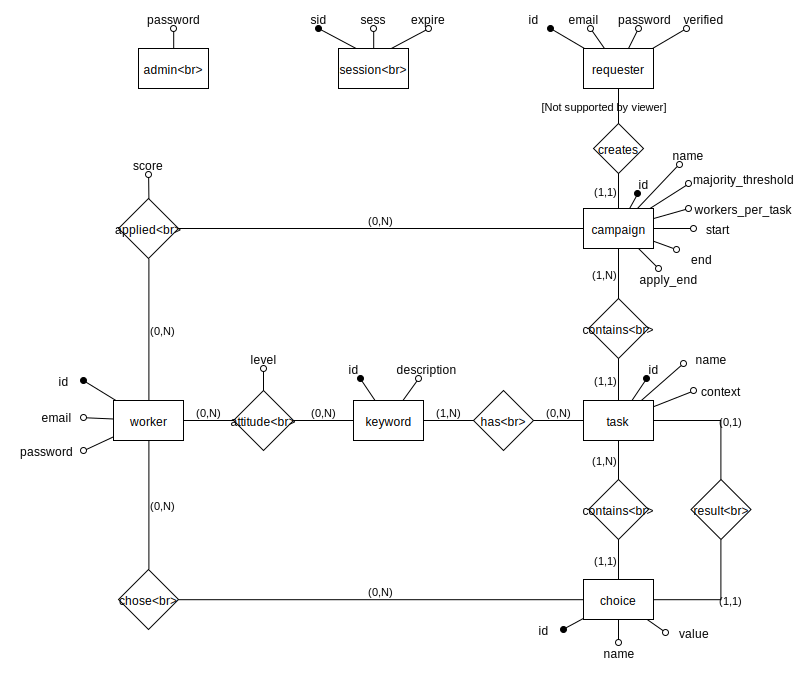
\includegraphics[width=\textwidth]{ER.png}
%\caption{ER}
\end{figure}

\subsubsection{Considerazioni su schema ER}
Ci sono tre tipologie di utenti, worker, requester e admin.
L'admin \`e un utente unico con nome utente predefinito e password modificabile, mentre il numero di worker e requester non \`e fissato. Hanno inoltre attributi simili, ma il requester ne presenta uno in pi\`u, e hanno relazioni diverse.

Quindi ho scelto di mantenere le entit\`a figlie invece di raggrupparle in un'entit\`a padre. Mantenendo cos\`i le singole tabelle.
Un motivo per cui ho fatto questa scelta \`e 
avere maggiore espressivit\`a dello schema della base di dati, poich\`e dal nome di della tabella \`e chiaro immediatamente a quale tipo di utente ci si riferisce.
Un'altra considarazione \`e che le interrogazioni discriminano sempre per tipo di utente, in quanto le relazioni sono diverse tra requester e worker. 
%Questa scelta \`e conseguenza delle seguenti due considerazioni: per risparmiare lo spazio di un attributo   sempre null dei worker; evitare una selezione in pi\`u per discriminare tra worker e requester.

Una scelta diversa \`e quella di raggruppare worker, requester e admin in un'entit\`a padre chiamata utente e discriminare a seconda dell'attributo \verb|tipo| che pu\`o assumere i valori ``worker'', ``requester'' o ``admin''.
Secondo me quest'ultima scelta avrebbe incrementato la complessit\`a delle interrogazioni.

\subsection{Schema relazionale}
Le chiavi esterne sono in corsivo e se non specificato tra parentesi si riferiscono all'attributo \verb|id| della tabella con lo stesso nome della chiave esterna.\\
Le chiavi primarie sono sottolineate.\\
Gli attributi opzionali sono indicati con un asterisco.
\\\\
requester(\underline{id}, email, password, verified)
\\
worker(\underline{id}, email, password)
\\
campaign(\uline{id}, name, majority\_threshold, workers\_per\_task, start, end, apply\_end, \textit{requester})
\\
task(\uline{id}, name, context, \textit{campaign}, \textit{result}$^*$(choice))
\\
choice(\uline{id}, name, value, \textit{task})
\\
keyword(\uline{id}, description)
\\
task\_keyword(\uline{\textit{task}, \textit{keyword}})
\\
worker\_attitude(\uline{\textit{worker}, \textit{keyword}}, level)
\\
worker\_campaign(\uline{\textit{worker}, \textit{campaign}}, score$^{*}$)
\\
worker\_choice(\uline{worker, choice})
\\
session(\uline{sid}, sess, expire)
\\
admin(password)

\subsection{Scelte progettuali}
\subsubsection{Gestione keyword}
Le keyword sono gestite con dei suggerimenti proposti al requester per la keyword che st\`a digitando.
I suggerimenti sono l'insieme delle keyword tali che l'input dell'utente ne \`e una sottostringa.
In questo modo l'utente ha tutta la liberta di scegliere le keyword che desidera tenendo sott'occhio le keyword ``simili'' gi\`a conosciute dall'applicazione.

Questa soluzione permette di evitare ridondanza dovuta all'uso del plurale e altri suffissi o prefissi.
La scelta di suggerire keyword che contengono l'input dell'utente come sottostringa \`e dovuta alla disponibilita dell'operatore sql \verb|like| e la sua semplicit\`a di utilizzo.

\subsubsection{Profilo lavoratore}
Il grado di competenza/attitudine di un lavoratore rispetto ad una keyword \`e rappresentato da un numero intero positivo.
Una keyword non associata al lavoratore si suppone abbia livello zero.
Tutti i lavoratori al momento dell'iscrizione, non hanno keyword associate e quindi hanno tutte le competenze/attitudini a livello zero.
Successivamente allo svolgimento di un task che risulta valido, vengono aggiornati i profili dei lavoratori che lo hanno eseguito, incrementando o decrementando di uno il livelo delle keyword associate al task.

Tutte le competenze/attitudini che si trovano a livello zero in un certo istante, vengono disassociate dal profilo del lavoratore in quanto il livello zero \`e sottinteso per tutte le keyword per tutti i lavoratori se non altrimenti specificato.

\subsubsection{Assegnazione task}
Responsabilit\`a della funzione pl/pgsql \verb|assign_task| nel file \verb|db/sql/1-functions.sql|.
\\\\
L'assegnazione di un task al lavoratore che ne fa richiesta all'interno di una campagna di lavoro \`e gestita mediante un indice detto $P$ calcolato per ogni task della  campagna di lavoro.

Dato un lavoratore che fa richiesta di un task, gli verr\`a assegnato il task con l'indice $P$ massimo tra i task non completati di quella campagna.
$$
P_{task} = \sum_{keyword \in task}{livello\_lavoratore(keyword)}
$$
Cio\`e, l'indice $P$ associato ad un generico task \`e la somma dei livelli delle keyword del task associate al lavoratore.

Per esempio un lavoratore appena iscritto ha tutte le competenze/attitudini a livello zero, quindi la scelta del task da assegnare diventa casuale.
Cosicch\`e al lavoratore non sia preclusa la possibilit\`a di eseguire dei task che non gli competono in parte o completamente. Al fine di permettere ai lavoratori di modellare in modo automatico il proprio profilo per rispecchiare il piu possibile la realt\`a.

\subsubsection{Aggiornamento profilo lavoratore}
Responsabilit\`{a} della funzione \verb|complete_task| nel file \verb|db/sql/1-functions.sql|.
\\\\
Questa funzione \`e attivata dal trigger per l'evento \verb|insert| della tabella \verb|worker_choice|, si occupa soprattutto di calcolare l'esito di un task e di aggiornare di conseguenza i profili dei lavoratori coinvolti qualora sia necessario.

Dato che tutti i lavoratori hanno tutte le keyword a livello zero se non altrimenti specificato.
L'aggiornamento del profilo di un lavoratore avviene incrementando o decrementando di uno il livello associato alla keyword, in base all'appartenenza del lavoratore al gruppo che ha dato la risposta maggioritaria.

Se la keyword viene decrementata al livello zero viene disassociata dal lavoratore e assume il suo valore di default, altrimenti, se la keyword viene incrementata a livello uno, dovra' essere associata al lavoratore esplicitamente in quanto possiede ora un livello maggiore di zero.

\subsubsection{Top 10 di una campagna di lavoro}
La classifica dei dieci migliori lavoratori di una campagna \`e decisa in base allo score dei lavoratori nella campagna stessa.

\section{Applicazione web}
\subsection{Connessione alla base di dati}
La connessione al database avviene attraverso la libreria nodeJs \emph{pg-promise}, che permette di effettuare interrogazioni asincrone con le \emph{Promesse} di javaScript.

\subsection{Backend}
Ho utilizzato la libreria \emph{express} per nodeJs perch\`e ritengo sia ideale per un'applicazione basata sulla base di dati. Principalmente perch\'e utizza il paradigma single thread, che permette di effettuare chiamate non bloccanti alla base di dati che gestisce il carico di lavoro.

\subsection{Frontend}
Sviluppato principalmente in HTML5, css\slash scss e javaScript.
Ho utilizzato la libreria css \emph{skeleton} per aiutarmi nello stile e nell'impaginazione, e la libreria javaScript \emph{awesomeplete} per il sistema di suggerimenti per le keyword durante la creazione di un task.

I sorgenti HTML sono nel formato di template \emph{Mustache},
per permettere la creazione dinamica delle pagine.



\end{document}
